\documentclass[11pt]{article}

\usepackage[margin=0.9in]{geometry}
\usepackage[T1]{fontenc}
\usepackage[utf8]{inputenc}
\usepackage{lmodern}
\usepackage{microtype}
\usepackage{amsmath,amssymb}
\usepackage{booktabs}
\usepackage{array}
\usepackage{tabularx}
\usepackage{graphicx}
\usepackage{xcolor}
\usepackage{tikz}
\usepackage{hyperref}
\usepackage{enumitem}

\usetikzlibrary{arrows.meta,positioning,fit,shapes.geometric}

\definecolor{ink}{HTML}{1D2530}
\definecolor{muted}{HTML}{586174}
\definecolor{line}{HTML}{C9D2DE}
\definecolor{blue}{HTML}{2563EB}
\definecolor{green}{HTML}{047857}
\definecolor{red}{HTML}{BE123C}
\definecolor{gold}{HTML}{A16207}
\definecolor{paper}{HTML}{FBFAF7}

\hypersetup{
  colorlinks=true,
  linkcolor=blue,
  citecolor=blue,
  urlcolor=blue,
  pdftitle={A Reproducible Kerr Force-Free Split-Monopole Gate},
  pdfauthor={Pim de Witte and the Lagra Project}
}

\setlist[itemize]{leftmargin=1.35em}
\setlist[enumerate]{leftmargin=1.55em}
\renewcommand{\arraystretch}{1.15}
\emergencystretch=2em

\newcommand{\code}[1]{\texttt{#1}}
\newcommand{\PsiBZ}{\ensuremath{\Psi_{\mathrm{BZ}}}}
\newcommand{\Residual}{\ensuremath{\mathcal{R}}}
\newcommand{\Order}[1]{\ensuremath{\mathcal{O}\!\left(#1\right)}}

\title{\textbf{A Reproducible Kerr Force-Free Split-Monopole Gate}\\
\large A Negative Finite-Spin Search Result and a Positive Blandford-Znajek Perturbative Anchor}
\author{Pim de Witte \\
Lagra Project / pde-engine adapter note}
\date{May 26, 2026}

\begin{document}
\maketitle

\begin{abstract}
We report a reproducible admission gate for candidate analytic solutions of a
closed Kerr force-free split-monopole Grad-Shafranov target.  The gate uses a
bounded pde-engine expression run, strict symbolic prechecks, a direct nonlinear
residual check, targeted finite-spin correction grammars, and a leading-order
coefficient solve.  The finite-spin search result is negative: 878 candidate
inputs were scanned, including 456 targeted finite-spin correction candidates
and 112 Kerr-metric-resummed correction candidates that passed the strict
prechecks before the full residual, and zero candidates had exact-zero
nonlinear residual.  A 48-coefficient leading-order ansatz produced 66
polynomial equations and SymPy returned \code{EmptySet}.  Separately, the same
gate recognizes the known slow-rotation Blandford-Znajek perturbative
split-monopole anchor: after substituting the Tanabe-Nagataki/Pan-Yu radial
correction and using $\operatorname{Li}_{1}(z)=-\log(1-z)$, the coefficient of
$a^2$ in the full residual simplifies exactly to zero.  This is a calibration
of the residual gate, not a claim of a new exact finite-spin Kerr solution.
\end{abstract}

\section{Claim}

The strongest result here is negative.  Under the implemented closed
split-monopole Kerr force-free target, the current bounded pde-engine search and
the targeted finite-spin correction families do not produce an admitted exact
finite-spin candidate.  The positive result is narrower but useful: the
residual implementation is not vacuous, because it accepts the established
\Order{a^2} Blandford-Znajek perturbative split-monopole correction as a
leading-order anchor.

\begin{center}
\resizebox{\linewidth}{!}{%
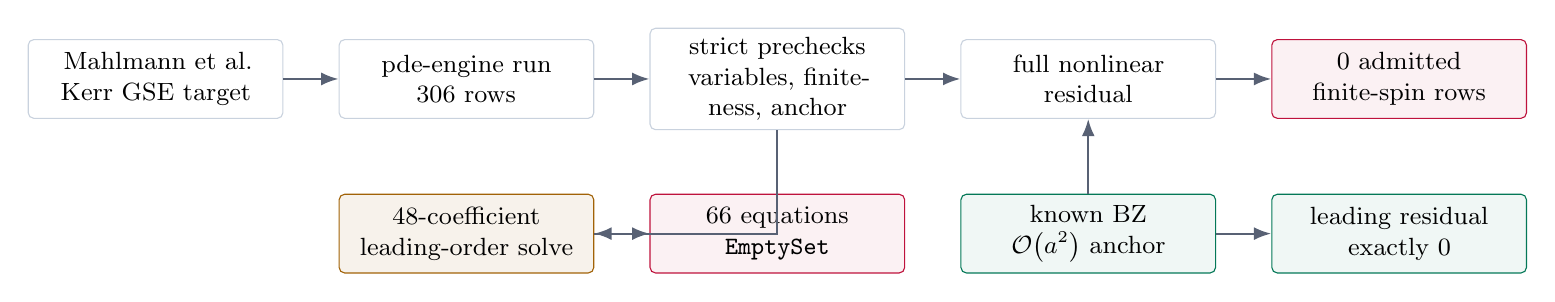
\begin{tikzpicture}[
  font=\small,
  node distance=0.65cm and 0.7cm,
  box/.style={draw=line, rounded corners=2pt, fill=white, align=center,
              minimum height=1.0cm, text width=3.0cm},
  good/.style={draw=green, fill=green!6},
  bad/.style={draw=red, fill=red!6},
  warn/.style={draw=gold, fill=gold!8},
  arrow/.style={-{Latex[length=2.2mm]}, thick, draw=muted}
]
  \node[box] (lit) {Mahlmann et al.\\Kerr GSE target};
  \node[box, right=of lit] (engine) {pde-engine run\\306 rows};
  \node[box, right=of engine] (pre) {strict prechecks\\variables, finiteness, anchor};
  \node[box, right=of pre] (res) {full nonlinear\\residual};
  \node[box, bad, right=of res] (zero) {0 admitted\\finite-spin rows};

  \draw[arrow] (lit) -- (engine);
  \draw[arrow] (engine) -- (pre);
  \draw[arrow] (pre) -- (res);
  \draw[arrow] (res) -- (zero);

  \node[box, warn, below=0.95cm of engine] (coeff) {48-coefficient\\leading-order solve};
  \node[box, bad, right=of coeff] (empty) {66 equations\\\code{EmptySet}};
  \draw[arrow] (coeff) -- (empty);
  \draw[arrow] (pre.south) |- (coeff.east);

  \node[box, good, below=0.95cm of res] (anchor) {known BZ\\\Order{a^2} anchor};
  \node[box, good, right=of anchor] (pass) {leading residual\\exactly 0};
  \draw[arrow] (anchor) -- (pass);
  \draw[arrow] (anchor.north) -- (res.south);
\end{tikzpicture}
}
\end{center}

\section{Literature Target}

The target equation is the stationary, axisymmetric, relativistic
Grad-Shafranov equation for force-free Kerr magnetospheres.  Mahlmann,
Cerda-Duran, and Aloy describe numerical solution techniques for this equation
in Kerr spacetimes and use established configurations such as split-monopole,
paraboloidal, black-hole-disk, and uniform field setups \cite{mahlmann2018}.
The reason this is a legitimate paper target is not that the equation is new;
it is that exact analytic finite-spin Kerr force-free solutions remain scarce.
Camilloni, Grignani, Harmark, Oliveri, and Orselli state the stronger boundary
used here: in the extreme Kerr case, there is no known exact analytic solution
to force-free electrodynamics that is stationary, axisymmetric, and
magnetically dominated \cite{camilloni2020}.

The gate closes the target with the split-monopole potential functions
\begin{align}
  r_+ &= M+\sqrt{M^2-a^2},\\
  \Omega(\Psi) &= \frac{a}{2(r_+^2+a^2)},\\
  I(\Psi) &= -\frac{\Omega}{2}\Psi(2-\Psi),\\
  II'(\Psi) &= I(\Psi)\frac{dI}{d\Psi}.
\end{align}
We write $x=\cos\theta$ and denote the implemented closed residual by
\begin{equation}
  \Residual[\Psi]\equiv
  \mathrm{GSLightCylinder}\!\left[\Psi;\Omega(\Psi),I(\Psi)\right].
\end{equation}
The exact expanded symbolic implementation is in
\path{tools/export_kerr_paper_target_gate.py}, in the function
\texttt{full\_\allowbreak kerr\_\allowbreak split\_\allowbreak monopole\_\allowbreak residual}.

\section{Admission Gate}

A row is admitted only if it passes all implemented gates below.  The order
matters.  Cheap symbolic filters run before the full nonlinear residual, so the
expensive residual simplification is not used to compensate for malformed
candidate expressions.

\begin{enumerate}
  \item The expression depends on $r$, $x$, and $a$.
  \item Denominators are finite on the rational safe points.
  \item The expression itself is finite on the same points.
  \item The $a\to 0$ limit is the Schwarzschild split-monopole anchor $1-x$ or
        the equivalent orientation $x$.
  \item The expression is not exactly one of the known anchors.
  \item The closed nonlinear residual $\Residual[\Psi]$ is exactly zero.
\end{enumerate}

The implemented gate deliberately does not yet prove global horizon,
axis, and light-surface regularity.  It also rejects exact known anchors but
does not yet implement a broad equivalence theory over gauge choices,
reparameterizations, and coordinate changes.  Those omissions matter for any
future positive claim; they do not weaken the negative statement made here.

\section{Bounded Search and Correction Families}

The source run was
\begin{center}
\begin{tabular}{ll}
\toprule
run id & \code{paper\_repro\_20260526\_104304\_2b096bdc}\\
problem & \code{kerr\_magnetosphere}\\
max depth & 2\\
validators & 1\\
per-expression timeout & 3.0 seconds\\
engine rows loaded & 306\\
completed validations & 306\\
\bottomrule
\end{tabular}
\end{center}

The exact reproduction command recorded by the artifact is
\begin{verbatim}
python3 tools/export_kerr_paper_target_gate.py \
  --run-engine --max-depth 2 --validators 1 \
  --timeout-s 90 --validation-timeout-s 3 --max-rows 1000
\end{verbatim}

The first targeted finite-spin grammar was
\begin{equation}
  \Psi = 1-x+a^2 c\,b(r,x),
  \qquad
  c\in\left\{-1,-\frac12,\frac12,1\right\},
\end{equation}
where $b(r,x)$ is a Cartesian product of eight angular factors and six radial
factors.  This produced 192 one-term candidates.  The two-term screen was
\begin{equation}
  \Psi = 1-x+a^2\left(c_1 b_i(r,x)+c_2 b_j(r,x)\right),
  \qquad c_1,c_2\in\{-1,1\},
\end{equation}
using a smaller 12-function sub-basis and unordered pairs.  This produced 264
two-term candidates.  All 456 targeted finite-spin corrections passed the
strict prechecks before the full residual.  None passed the full residual.

The follow-up search added a Kerr-metric-resummed screen.  It preserves the
same $a\to0$ split-monopole anchor but permits finite-spin denominators built
from the metric factors
\begin{equation}
  \Sigma = r^2+a^2x^2,\qquad
  \Delta = r^2-2Mr+a^2,\qquad
  A = (r^2+a^2)^2-\Delta a^2(1-x^2).
\end{equation}
The screen has the form
\begin{equation}
  \Psi = 1-x+a^2 c\,m(r,x,a,M),
  \qquad
  c\in\left\{-1,-\frac12,\frac12,1\right\},
\end{equation}
with four anchor-preserving angular factors and seven metric radial/denominator
factors.  This generated 112 additional candidates.  All 112 passed the strict
prechecks before the full residual.  None passed the full residual.

\begin{center}
\resizebox{\linewidth}{!}{%
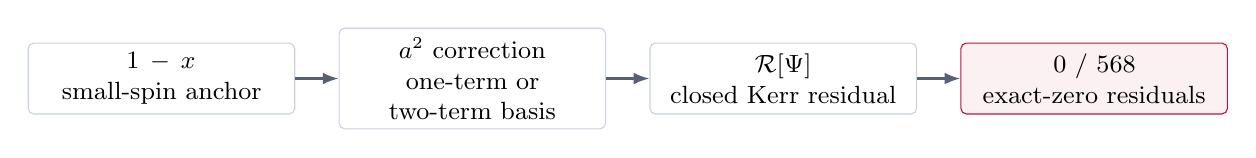
\begin{tikzpicture}[
  font=\small,
  node distance=0.55cm,
  piece/.style={draw=line, rounded corners=2pt, fill=white,
                align=center, minimum height=0.9cm, text width=3.15cm},
  arrow/.style={-{Latex[length=2mm]}, thick, draw=muted}
]
  \node[piece] (anchor) {$1-x$\\small-spin anchor};
  \node[piece, right=of anchor] (corr) {$a^2$ correction\\one-term or two-term basis};
  \node[piece, right=of corr] (gate) {$\Residual[\Psi]$\\closed Kerr residual};
  \node[piece, right=of gate, draw=red, fill=red!6] (out) {0 / 568\\exact-zero residuals};
  \draw[arrow] (anchor) -- (corr);
  \draw[arrow] (corr) -- (gate);
  \draw[arrow] (gate) -- (out);
\end{tikzpicture}
}
\end{center}

\section{Coefficient Solve}

The sampled coefficients above are only a finite screen.  To avoid mistaking
that for a proof about the one-term basis, the gate also solves the leading
coefficient system
\begin{equation}
  \Psi = 1-x+a^2\sum_{i=1}^{48} c_i b_i(r,x), \qquad M=1,
\end{equation}
and expands the residual as
\begin{equation}
  \Residual[\Psi] = a^2 P(r,x;\mathbf{c})+\Order{a^4}.
\end{equation}
After denominator clearing, the polynomial identity $P=0$ gives 66 equations
in 48 unknowns.  SymPy reports
\begin{equation}
  \mathrm{linsolve}(A\mathbf{c}=0)=\varnothing.
\end{equation}
Thus the one-term ansatz family has no leading-order correction within this
basis; it is not merely that four sampled coefficient values failed.

\section{Perturbative Blandford-Znajek Anchor}

The calibration screen inserts the known slow-rotation split-monopole
correction from the Blandford-Znajek perturbative literature.  Tanabe and
Nagataki analyze higher-order terms for the Kerr-parameter expansion and
emphasize that the known analytic monopole solution is perturbative through
second order in spin \cite{tanabe2008}.  Pan and Yu extend the split-monopole
perturbation solution to fourth order and likewise identify the second-order
split-monopole solution as the known analytic Blandford-Znajek baseline
\cite{pan2015}.

With $M=1$, the gate inserts
\begin{equation}
  \PsiBZ = 1-x+a^2x(1-x^2)R(r),
\end{equation}
where
\begin{align}
R(r) ={}&
\frac{r^2(2r-3)}{8}
\left[
  \operatorname{Li}_2\!\left(\frac{2}{r}\right)
  -\log\!\left(1-\frac{2}{r}\right)\log\!\left(\frac{r}{2}\right)
\right] \notag\\
&+\frac{1+3r-6r^2}{12}\log\!\left(\frac{r}{2}\right)
  +\frac{11}{72}+\frac{1}{3r}+\frac{r}{2}-\frac{r^2}{2}.
\end{align}
The check is
\begin{equation}
  [a^2]\,\Residual[\PsiBZ] = 0,
\end{equation}
where the residual is series-expanded through \Order{a^4}.  The symbolic
normalization uses the identity
\begin{equation}
  \operatorname{Li}_{1}(z)=-\log(1-z).
\end{equation}
After that replacement, the leading residual simplifies exactly to zero, and
all rational point checks are zero.  The artifact records this as
\texttt{passes\_\allowbreak leading\_\allowbreak order\_\allowbreak anchor}.  It also records
\texttt{finite\_\allowbreak spin\_\allowbreak exact\_\allowbreak candidate=false}.  That flag is not cosmetic:
\(\PsiBZ\) is a perturbative \Order{a^2} anchor and must not be reported as a
new exact finite-spin solution.

\section{Results}

The machine-readable artifact status is \code{no\_candidate\_yet}.  That status
is not a failure of the gate; it is the correct output when the gate is
implemented and no candidate in scope passes it.

\begin{center}
\begin{tabularx}{0.98\linewidth}{>{\raggedright\arraybackslash}p{0.34\linewidth}
                                >{\raggedright\arraybackslash}p{0.18\linewidth}
                                >{\raggedright\arraybackslash}X}
\toprule
Screen & Status & Evidence \\
\midrule
engine generation & implemented & 306 generated rows loaded for the strict gate. \\
strict prechecks & implemented & candidate variables, finite denominators, finite values, small-spin anchor, and exact-anchor rejection recorded per row. \\
full nonlinear residual & implemented negative & 0 exact-zero residual rows; admitted count 0. \\
bounded correction screens & implemented negative & 192 one-term and 264 two-term corrections; 456 passed strict prechecks; 0 passed the full residual. \\
metric-resummed screen & implemented negative & 112 Kerr-metric-denominator corrections; 112 passed strict prechecks; 0 passed the full residual. \\
coefficient solve & no leading-order solution & 66 equations, 48 unknowns, matrix shape [66,48], \code{EmptySet}. \\
literature perturbative anchor & passes leading-order anchor & Tanabe-Nagataki/Pan-Yu \Order{a^2} correction gives exact-zero leading residual. \\
equivalence filters & partial & exact known anchors rejected; broad gauge/reparameterization equivalence remains future work. \\
global regularity & not sufficient for positive claim & rational safe-point checks exist; global horizon, axis, and light-surface proofs are not implemented. \\
\bottomrule
\end{tabularx}
\end{center}

The paper result is therefore:
\begin{equation}
  \boxed{\text{finite-spin exact Kerr candidate: not found}}
  \qquad
  \boxed{\text{known \Order{a^2} BZ perturbative anchor: recovered}}.
\end{equation}

\section{Reproducibility}

The machine-readable source of truth is
\path{docs/kerr-paper-target-gate.json}.  The human-readable gate summary is
\path{docs/kerr-paper-target-gate.md}.  The implementation and tests are:
\begin{itemize}
  \item \path{tools/export_kerr_paper_target_gate.py}
  \item \path{tests/test_kerr_paper_target_gate.py}
\end{itemize}
The relevant regression asserts that the literature slow-rotation anchor is
enabled, has status
\texttt{passes\_\allowbreak leading\_\allowbreak order\_\allowbreak anchor}, has
\texttt{leading\_\allowbreak residual\_\allowbreak exact\_\allowbreak zero=true},
has simplified residual \code{0},
and is not a finite-spin exact candidate.

The verification bundle used for the current artifact included Python syntax
checks, the force-free and Kerr unit tests, JSON validation, PDF text checks,
the Lean normalizer build, and Git whitespace hygiene.  The generated SQLite
run outputs and validator caches are intentionally not part of the paper
claim; they are local execution artifacts.

\section{Conclusion}

The work converts an ambiguous search program into an executable scientific
gate.  The gate currently rejects every generated or targeted finite-spin
candidate in scope.  This is a meaningful negative result because the same
residual implementation accepts the known Blandford-Znajek slow-rotation
perturbative correction at leading order.  The next publishable positive paper
would need a candidate that passes the exact residual, stronger equivalence
filters, and global regularity checks.  This paper does not claim that such a
candidate has been found.

\begin{thebibliography}{9}

\bibitem{mahlmann2018}
J. F. Mahlmann, P. Cerda-Duran, and M. A. Aloy,
\emph{Numerically solving the relativistic Grad-Shafranov equation in Kerr
spacetimes: numerical techniques},
Monthly Notices of the Royal Astronomical Society 477, 3927--3945 (2018),
\href{https://arxiv.org/abs/1802.00815}{arXiv:1802.00815}.

\bibitem{camilloni2020}
F. Camilloni, G. Grignani, T. Harmark, R. Oliveri, and M. Orselli,
\emph{Moving away from the Near-Horizon Attractor of the Extreme Kerr
Force-Free Magnetosphere},
JCAP 10, 048 (2020),
\href{https://arxiv.org/abs/2007.15665}{arXiv:2007.15665}.

\bibitem{tanabe2008}
K. Tanabe and S. Nagataki,
\emph{Extended monopole solution of the Blandford-Znajek mechanism: Higher
order terms for a Kerr parameter},
Physical Review D 78, 024004 (2008),
\href{https://doi.org/10.1103/PhysRevD.78.024004}{doi:10.1103/PhysRevD.78.024004},
\href{https://arxiv.org/abs/0802.0908}{arXiv:0802.0908}.

\bibitem{pan2015}
Z. Pan and C. Yu,
\emph{Fourth-order split monopole perturbation solutions to the
Blandford-Znajek mechanism},
Physical Review D 91, 064067 (2015),
\href{https://doi.org/10.1103/PhysRevD.91.064067}{doi:10.1103/PhysRevD.91.064067},
\href{https://arxiv.org/abs/1503.05248}{arXiv:1503.05248}.

\end{thebibliography}

\end{document}
